\documentclass[11pt]{article}
\usepackage{classTools}
\usepackage{tikz}
\usepackage{chessboard}
\usepackage{xcolor}
\usepackage{float}

\begin{document}

% To include a problems set header, use the psHeader command
\psHeader{5}{Wed Oct. 23, 2024 (11:59pm)}

\textbf{Your name: Roshen Chatwal}

\textbf{Collaborators: Raunak Daga}

\textbf{No. of late days used on previous psets: 1-ish }

\textbf{No. of late days used after including this pset: 1}

\medskip \noindent
\textit{Remember to mark your pages on Gradescope properly, or points will be taken off. Additionally, if your handwriting isn't particularly neat please submit written proofs, which are much easier to grade for the TFs.}

\begin{enumerate}
    \item (Solving Games) Consider playing a solo game on an $n\times n$ chessboard.  You have one piece, a chess knight, which starts in the lower-left corner, and your goal is to reach any of the other three corners in as few moves as possible.  Like a usual chess knight, in one move, you can move to any position that is two squares away in a horizontal direction and one square away in a vertical direction, or two squares away in a vertical direction and one square away in a horizontal direction.  There is a catch, however: some squares have visible landmines, so you cannot move to them (since you do not want set off an explosion). \ 

    \begin{enumerate}
    \item Give an algorithm that achieves the above goal in time $O(n^2)$ by reduction to either the ShortestWalks problem or the SingleSourceShortestPaths problem. The algorithm should output $\bot$ if no sequence of moves can take you to any of the other three corners when started in the lower-left corner. (Note: if reducing to SingleSourceShortestPaths, we haven't defined abstractly what it means to reduce a computational problem to a data structure problem, but you may construct and use a SingleSourceShortestPaths data structure on an appropriately constructed graph.) \\

    I will give an algorithm that achieves the goal above in time $O(n^2)$ by reduction to the ShortestWalks problem and then prove its correctness and justify its runtime. \\

\textbf{Preprocessing: Making a graph G} \\

Construct an undirected graph $G = (V,E)$, with the nodes being squares and the edges being connections between nodes that are a valid knight's move away from each other. On an implementation level, we can do this for an $n \times n$ board $B$ containing landmines by doing: \\

\begin{verbatim}
for i in range(n): 
    for j in range(n): 
        - skip this iteration and move on to the next nested loop 
          if there's a landmine on square B[i][j]
        - find all the squares s in B that are one "L" away 
          (two squares away in a horizontal direction and one square 
          away in a vertical direction, or two squares away in a vertical 
          direction and one square away in a horizontal direction) 
          from square B[i][j] per the knight's moving rules and 
          store in a temporary array
        - check each square s in the temporary array for the presence 
          of a landmine and delete the ones with landmines from 
          the temporary array
        - for each square s remaining in the temporary array 
            - if s is not already in the set of vertices V:
                - add s to the set of vertices, V, in the graph G
            - add the edge (B[i][j], s) to the set of edges, E, in the graph G
\end{verbatim} \\

\textbf{Oracle: BFS variant} \\
Let $x$ be the bottom-left square of the board $B$ (at location $B[0][0]$ per my definition of $B$). Run the variant of $BFS(G, x)$ that also makes an array of which vertex precedes each vertex in our walk sequentially if that vertex was reached in the walk and has some null value otherwise (AKA put the number of the vertex $y$ at index $z$ in the array if we arrived at $y$ immediately before arriving at $z$). Essentially, the oracle will give us two arrays $A$ and $B$, where $A$ is the array containing the distance between vertices $x$ and $y$ at $A[y]$ and $B$ is the array containing $y$ at $B[z]$ if vertex $y$ immediately precedes vertex $z$ in the walk. For ease later on, we can modify $BFS$ to initialize the arrays $A$ and $B$ to size $n^2$ initially instead of the number of vertices in G since G won't have all the squares in B (only the ones that are accessible from non-landmine squares and that aren't landmines themselves). Each initial value in $A$ can be assigned to $\infty$ and each initial value in $B$ can be assigned to "Null", as our BFS variant will only assign finite distances and predecessors on a walk of finite length between $x$ and the vertices in G at relevant indices of $A$ and $B$. Essentially, I just set the size of the G in preprocessing to the bare minimum (wouldn't have done so if y'all didn't make me do the algo by hand in part 1b) while pretending it has $n^2$ vertices for ease with BFS and postprocessing.\\

\textbf{Postprocessing and Outputs: Getting our three shortest walks} \\
It's pretty simple, using our arrays $A$ and $B$. Let $a$, $b$, and $c$ represent the squares at the top-left, top-right, and bottom-right squares, respectively (AKA $B[0][n-1]$, $B[n-1][n-1]$, and $B[n-1][0]$, respectively). First, we check $A[s]$ for each $s \in \{a, b, c\}$, and return $\bot$ if all $A[s] = \infty$ because that means there aren't sequences of moves that can take us to any of the other three corners when started in the lower-left corner (due to landmines blocking what would otherwise be the path or the corner itself having a landmine). \\
If we haven't returned $\bot$ by now, it means that there does exist a walk that can take us to at least one of the other three corners when started in the lower-left corner. To find the possible walks, we can initialize three empty arrays $C_a$, $C_b$, and $C_c$ (assuming $a, b, c$ are accessible otherwise we can initialize fewer arrays only for the sequences to accessible corners). Then, for each $s \in \{a, b, c\}$ (assuming all other corners are accessible once again, but there will be fewer values of $s$ if not), we parse through array $B$ and collect nodes on the reverse path from $x$ to $s$. We start by adding $s$ to array $C_s$. Then, we look at $B[s]$, adding the value there $v$ to array $C_s$, and then look at $B[v]$. We repeat this backward and reverse-path development in each $C_s$ until we have added $x$ to $C_s$ (which means we got all the way back to our starting square $x$). At this point, each $C_s$ has the sequence of vertices we reach on our shortest path from $x$ to $s$, but in reverse. Thus, we simply need to reverse the order of each $C_s$ to achieve our goal of finding the shortest sequence of moves needed for a knight to move from $x$ to $s$ $\forall  s \in \{a, b, c\}$ (assuming each corner is accessible again, but there'd be fewer in the set if not)! We return each reversed $C_s$ as the output, which is all possible paths from $x$ to another corner of the board when such a path exists. Note that a particular $C_s$ could come in multiple valid forms if there exists multiple distinct shortest walks between $x$ and $s$ (as is the case in the example below).\\

\textbf{Correctness: } \\
If there exists a path from $x$ to $s$ for some $s \in \{a, b, c\}$, my algorithm will give the correct paths between $x$ and $s$ because the creation of graph $G$ includes only the valid vertices the knight can reach and paths the knights can tread when starting at the lower-left corner. By the correctness of BFS, we know that $A$ will contain the shortest distances between $x$ and $s$ and the variant will consequentially give us the predecessor to a vertex $v$ on our shortest walk. Thus, the reverse of our arrays $C_s$ will contain the sequence of vertices that we'll tread on the shortest walk from $x$ to $s$. \\
If there doesn't exist a path from $x$ to $s$ for $\forall s \in \{a, b, c\}$, my algorithm will correctly return $\bot$ due to the correctness of BFS, which ensures $A[v] = \infty$ for all $v$ that can't possibly be reached on the knight's path (AKA $v$ that are in a different connected component of $G$ from $x$ or $v$ containing landmines that just aren't in G). \\

\textbf{Runtime analysis:} \\
Preprocessing takes $O(n^2)$ time to make the graph. We're iterating over each of the $n^2$ squares, and it takes a constant number of steps to find/store any newly found landing squares and paths in the knight's range of motion from a particular square (because there's up to 8 valid squares a knight can move to from a particular square and inserting those squares/edges into $G$ also takes a constant number of steps). \\
The oracle takes $O(1)$ time in the runtime of our reduction. \\
Postprocessing takes $O(n^2)$ time. Checking each $A[s]$ for whether it equals $\infty$ takes $3 \cdot O(1) = O(1)$ time, making our arrays $C_s$ take $3 \cdot O(n^2)$ time because we'll backward-traverse no more than $n^2$ locations in $B$ and insertion into $C_s$ takes $O(1)$ steps, and reversing the $C_s$ arrays to get our final sequences from $x$ to $s$ takes $3 \cdot O(n^2) = O(n^2)$ time since there's no more than $n^2$ elements in our arrays. So all in all, post processing takes $O(n^2)$ time. \\
Aggregating the steps above, the runtime of this reduction takes $O(n^2) + O(1) + O(n^2) = O(n^2)$ time. Thus, I've described a correct reduction from our goal to the ShortestWalks problem that takes $O(n^2)$ time, using a variant of BFS as the oracle. \\

    \item Carry out your algorithm on the $5\times 5$ board shown below, listing both the frontier vertices and the predecessor relationships at each stage of BFS (the red square symbols are landmines).
    
    \begin{figure} [H]
    \centering
    \begin{tikzpicture}
        \definecolor{white}{rgb}{1,1,1}
        \definecolor{black}{rgb}{0.5,0.5,0.5}
        \definecolor{darkred}{rgb}{0.6, 0, 0}

        \def\landmines{(2.5,1.5), (1.5,5.5), (5.5,1.5), (1.5,3.5), (3.5,1.5),(3.5,3.5),(4.5,4.5),(4.5,5.5),(2.5,4.5), (4.5,3.5)}
        
        % Loop to create the 5x5 grid
        \foreach \x in {1,...,5} {
            \foreach \y in {1,...,5} {
                % Alternate black and white squares
                \pgfmathparse{mod(\x+\y,2)}
                \ifnum\pgfmathresult=0
                    \fill[white] (\x, \y) rectangle ++(1,1);
                \else
                    \fill[black] (\x, \y) rectangle ++(1,1);
                \fi
            }
        }
    
        % X-axis labels
        \foreach \x/\letter in {1/a, 2/b, 3/c, 4/d, 5/e} {
            \node at (\x+0.5, 0.5) {\letter}; 
        }
    
        % Y-axis labels
        \foreach \y in {1, 2, 3, 4, 5} {
            \node at (0.5, \y+0.5) {\y};  
        }
    
        % Knight symbol
        \node at (1.5, 1.5) {\knight};

        %Adding landmines
        \foreach \position in \landmines {
            \draw[fill=red, opacity=0.5] \position ++(-0.3,-0.3) rectangle ++(0.6,0.6); 
            \node at \position {\textcolor{darkred}{\Huge$\circ$}};  
        }
    
        % Grid lines
        \draw[step=1cm,black,thick] (1,1) grid (6,6);
        
    \end{tikzpicture}
    \end{figure}

    \end{enumerate} \\

    This took soooo long I wish I knew I didn't have to go this in depth \\

\begin{figure}[H]
    \centering
    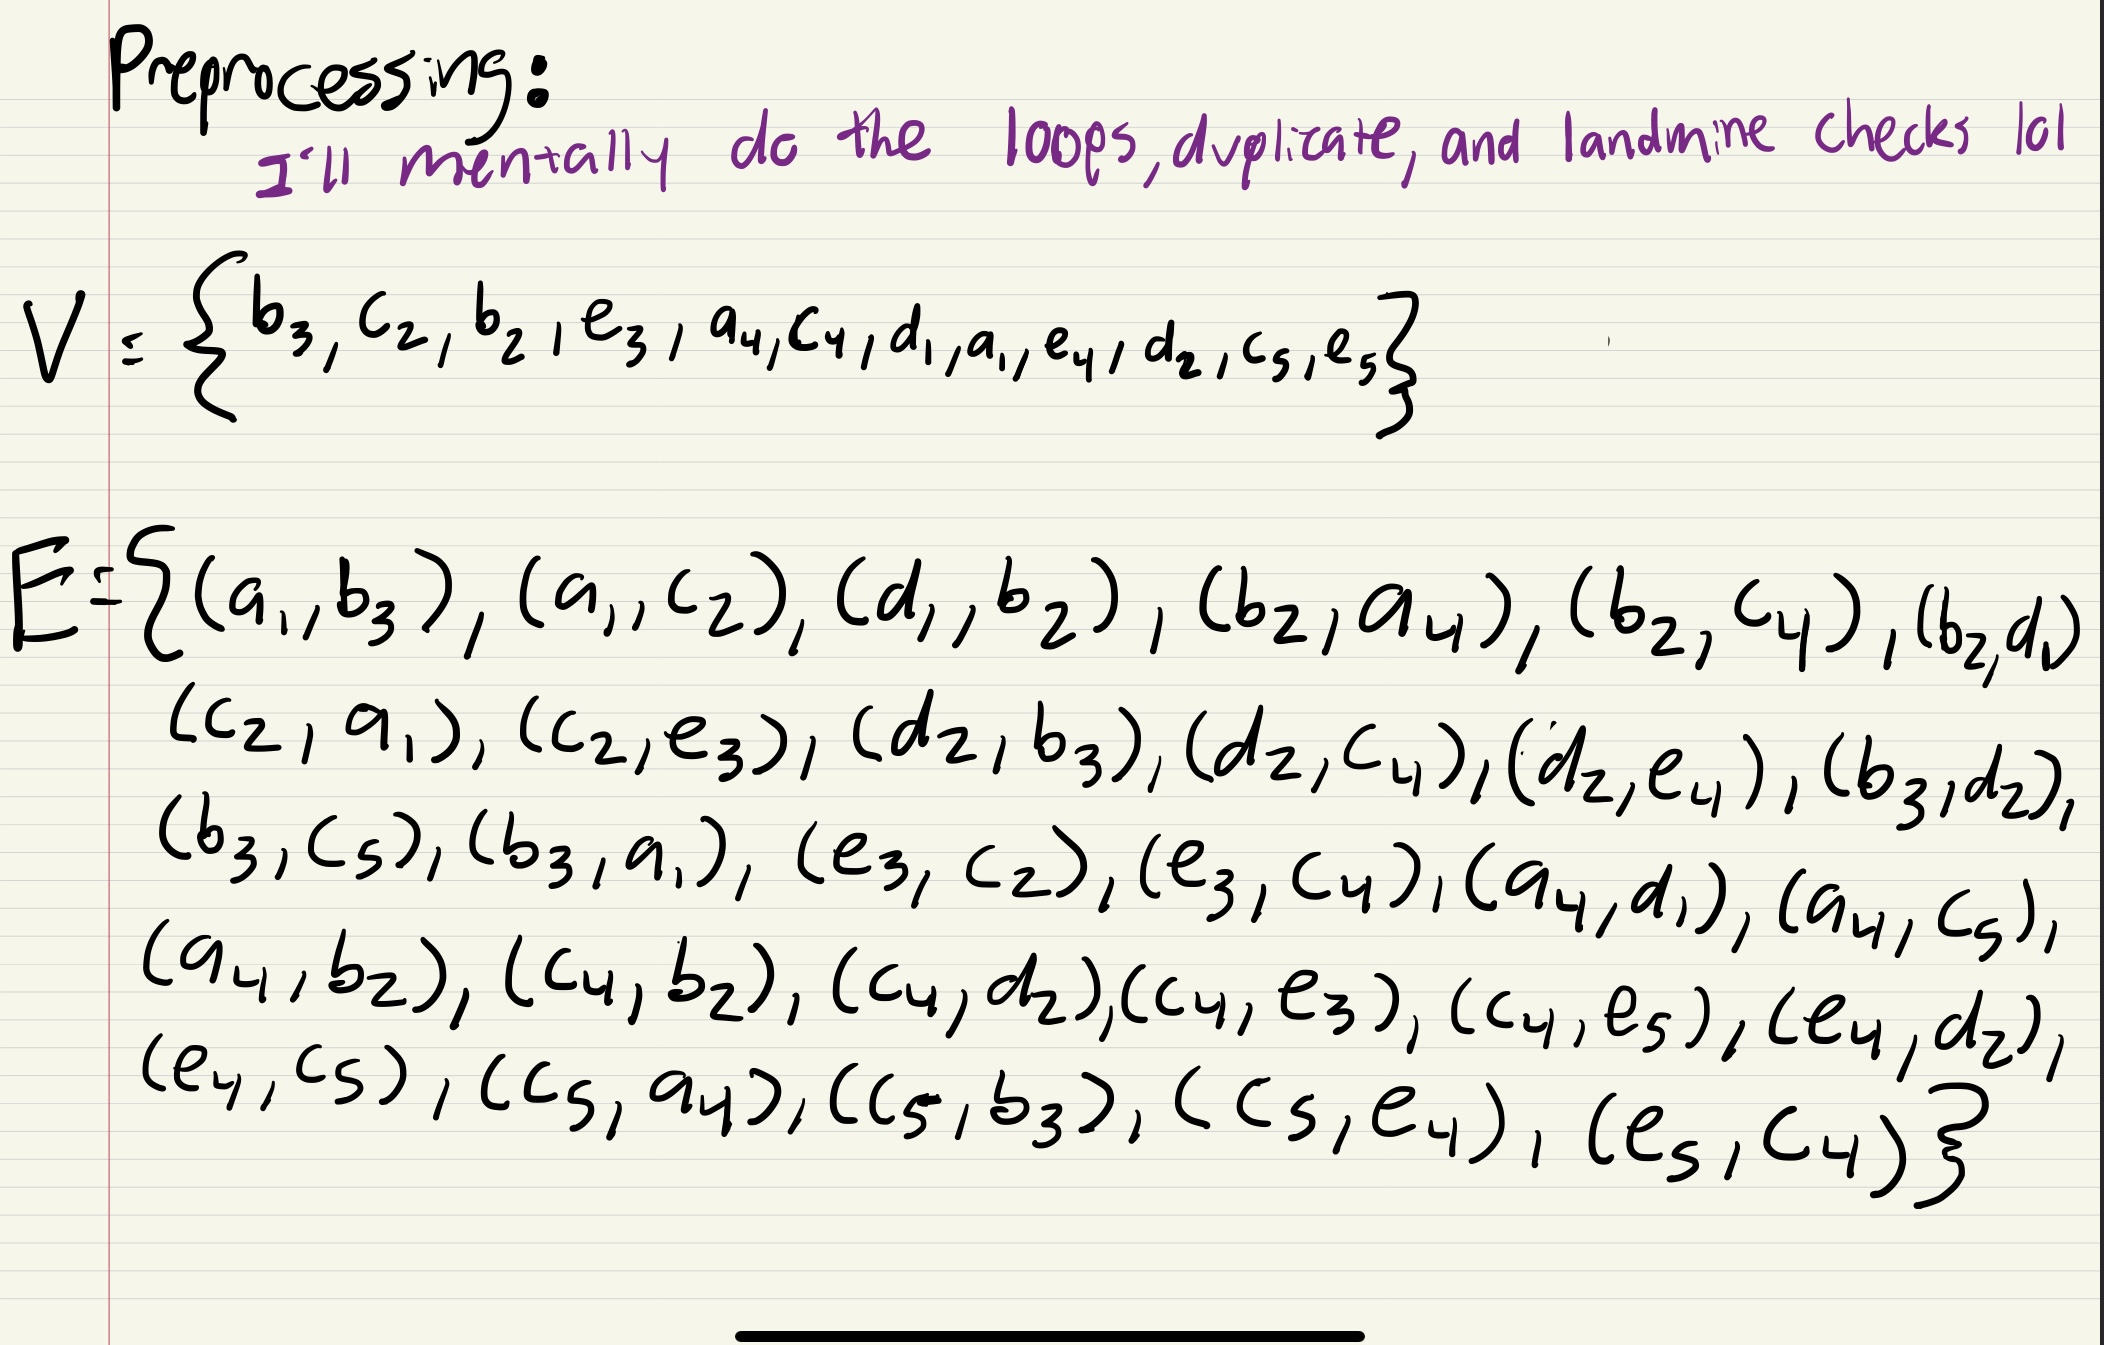
\includegraphics[width=.75\linewidth]{IMG_0130.jpg}
    \caption{Preprocess}
    \label{fig:preprocess}
\end{figure}

\begin{figure}[H]
    \centering
    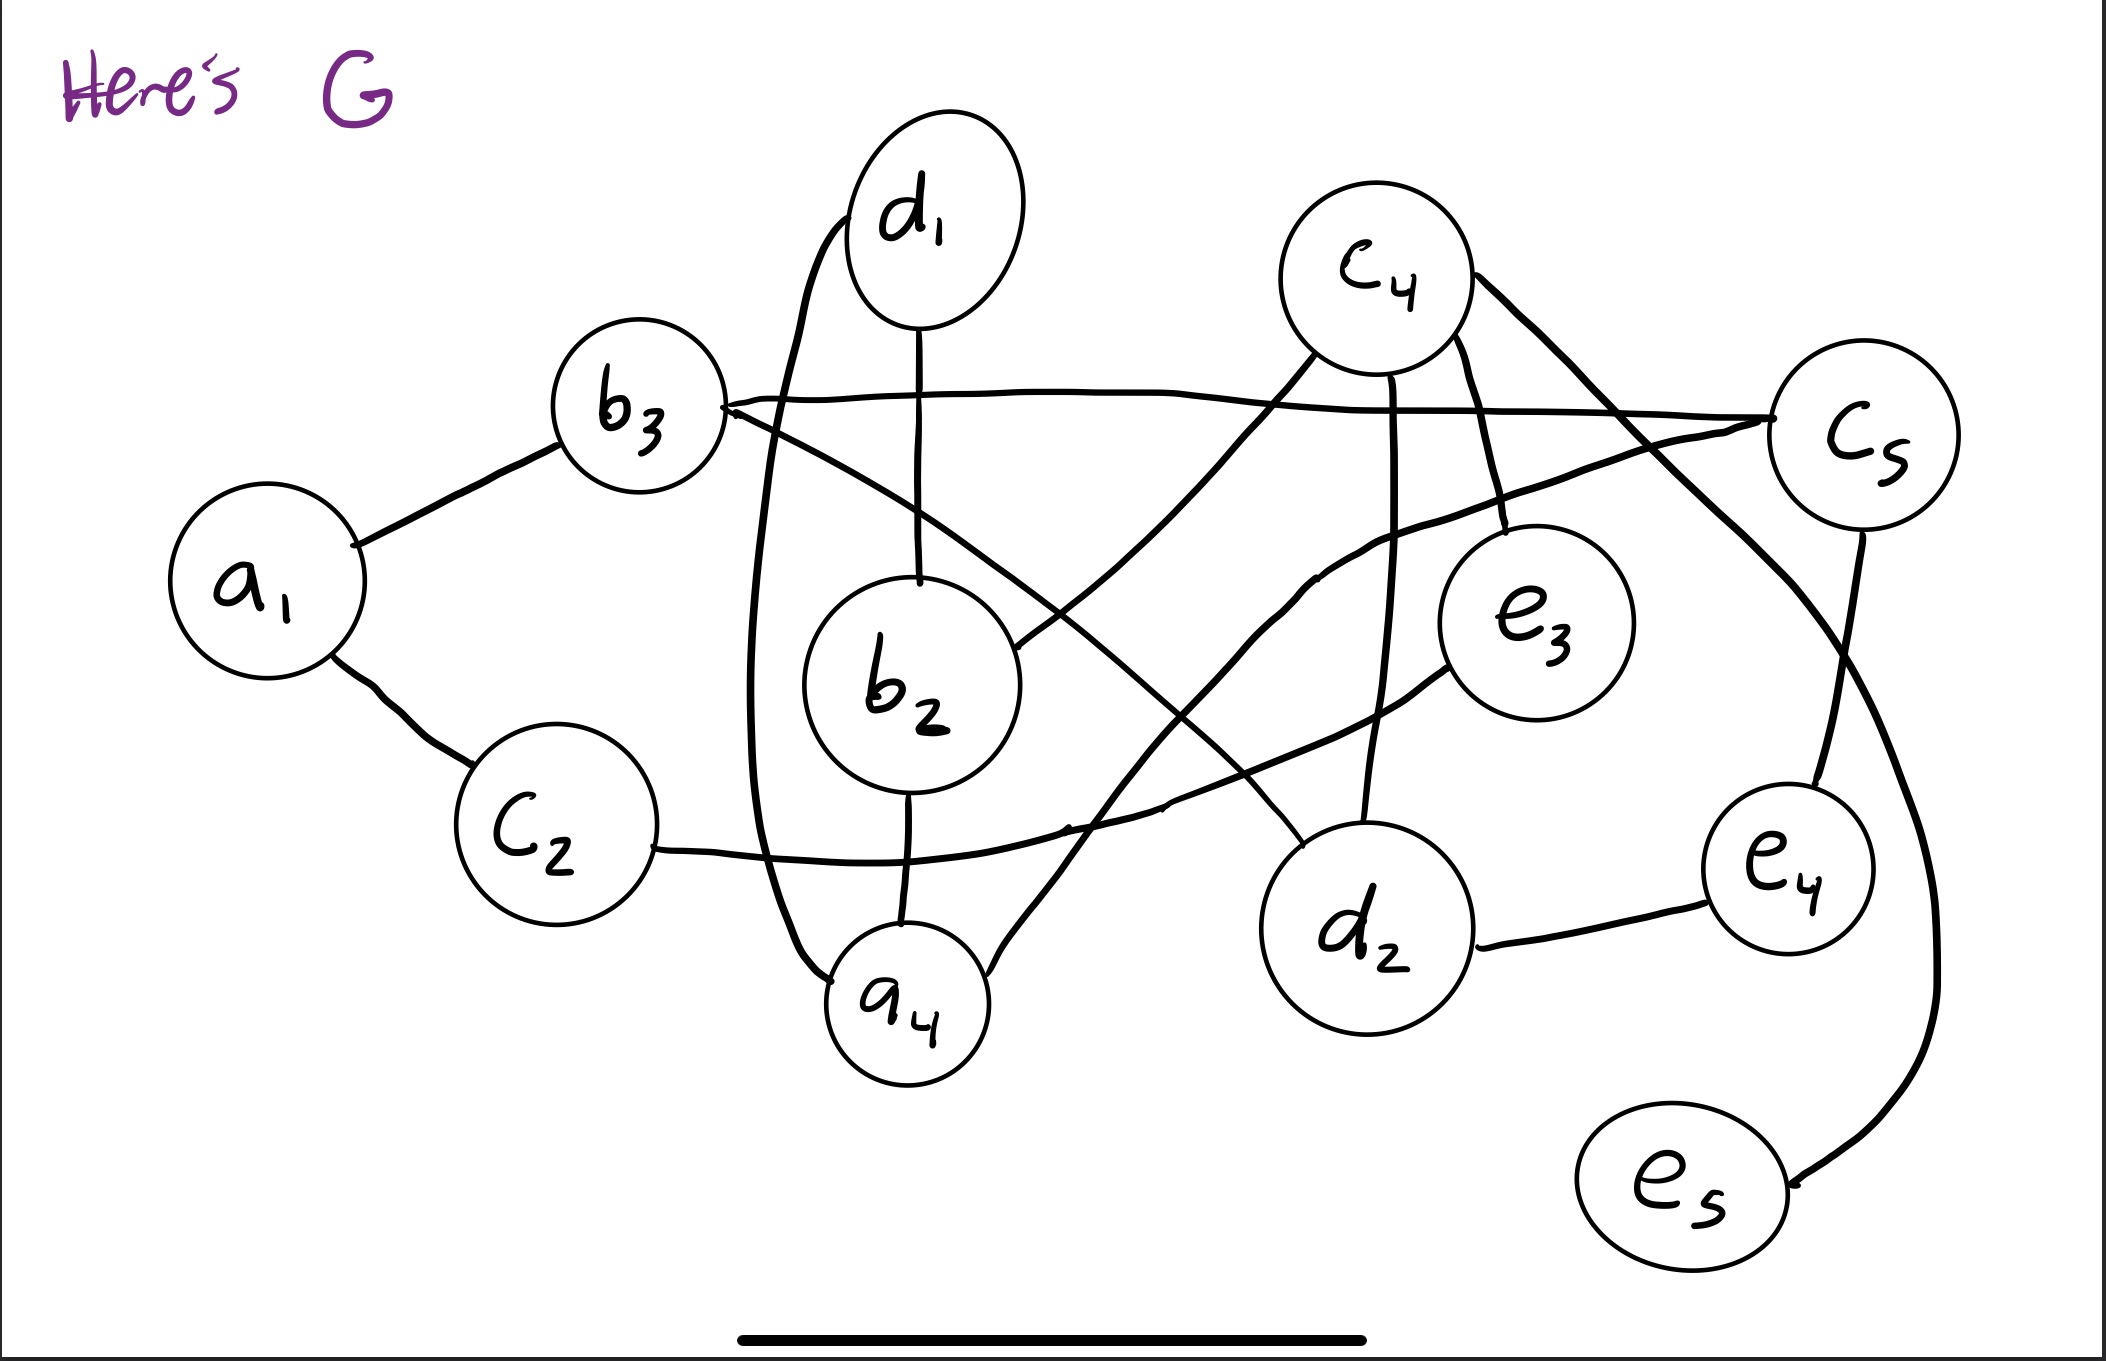
\includegraphics[width=.75\linewidth]{IMG_0131.jpg}
    \caption{Graph}
    \label{fig:graph}
\end{figure}

\begin{figure}[H]
    \centering
    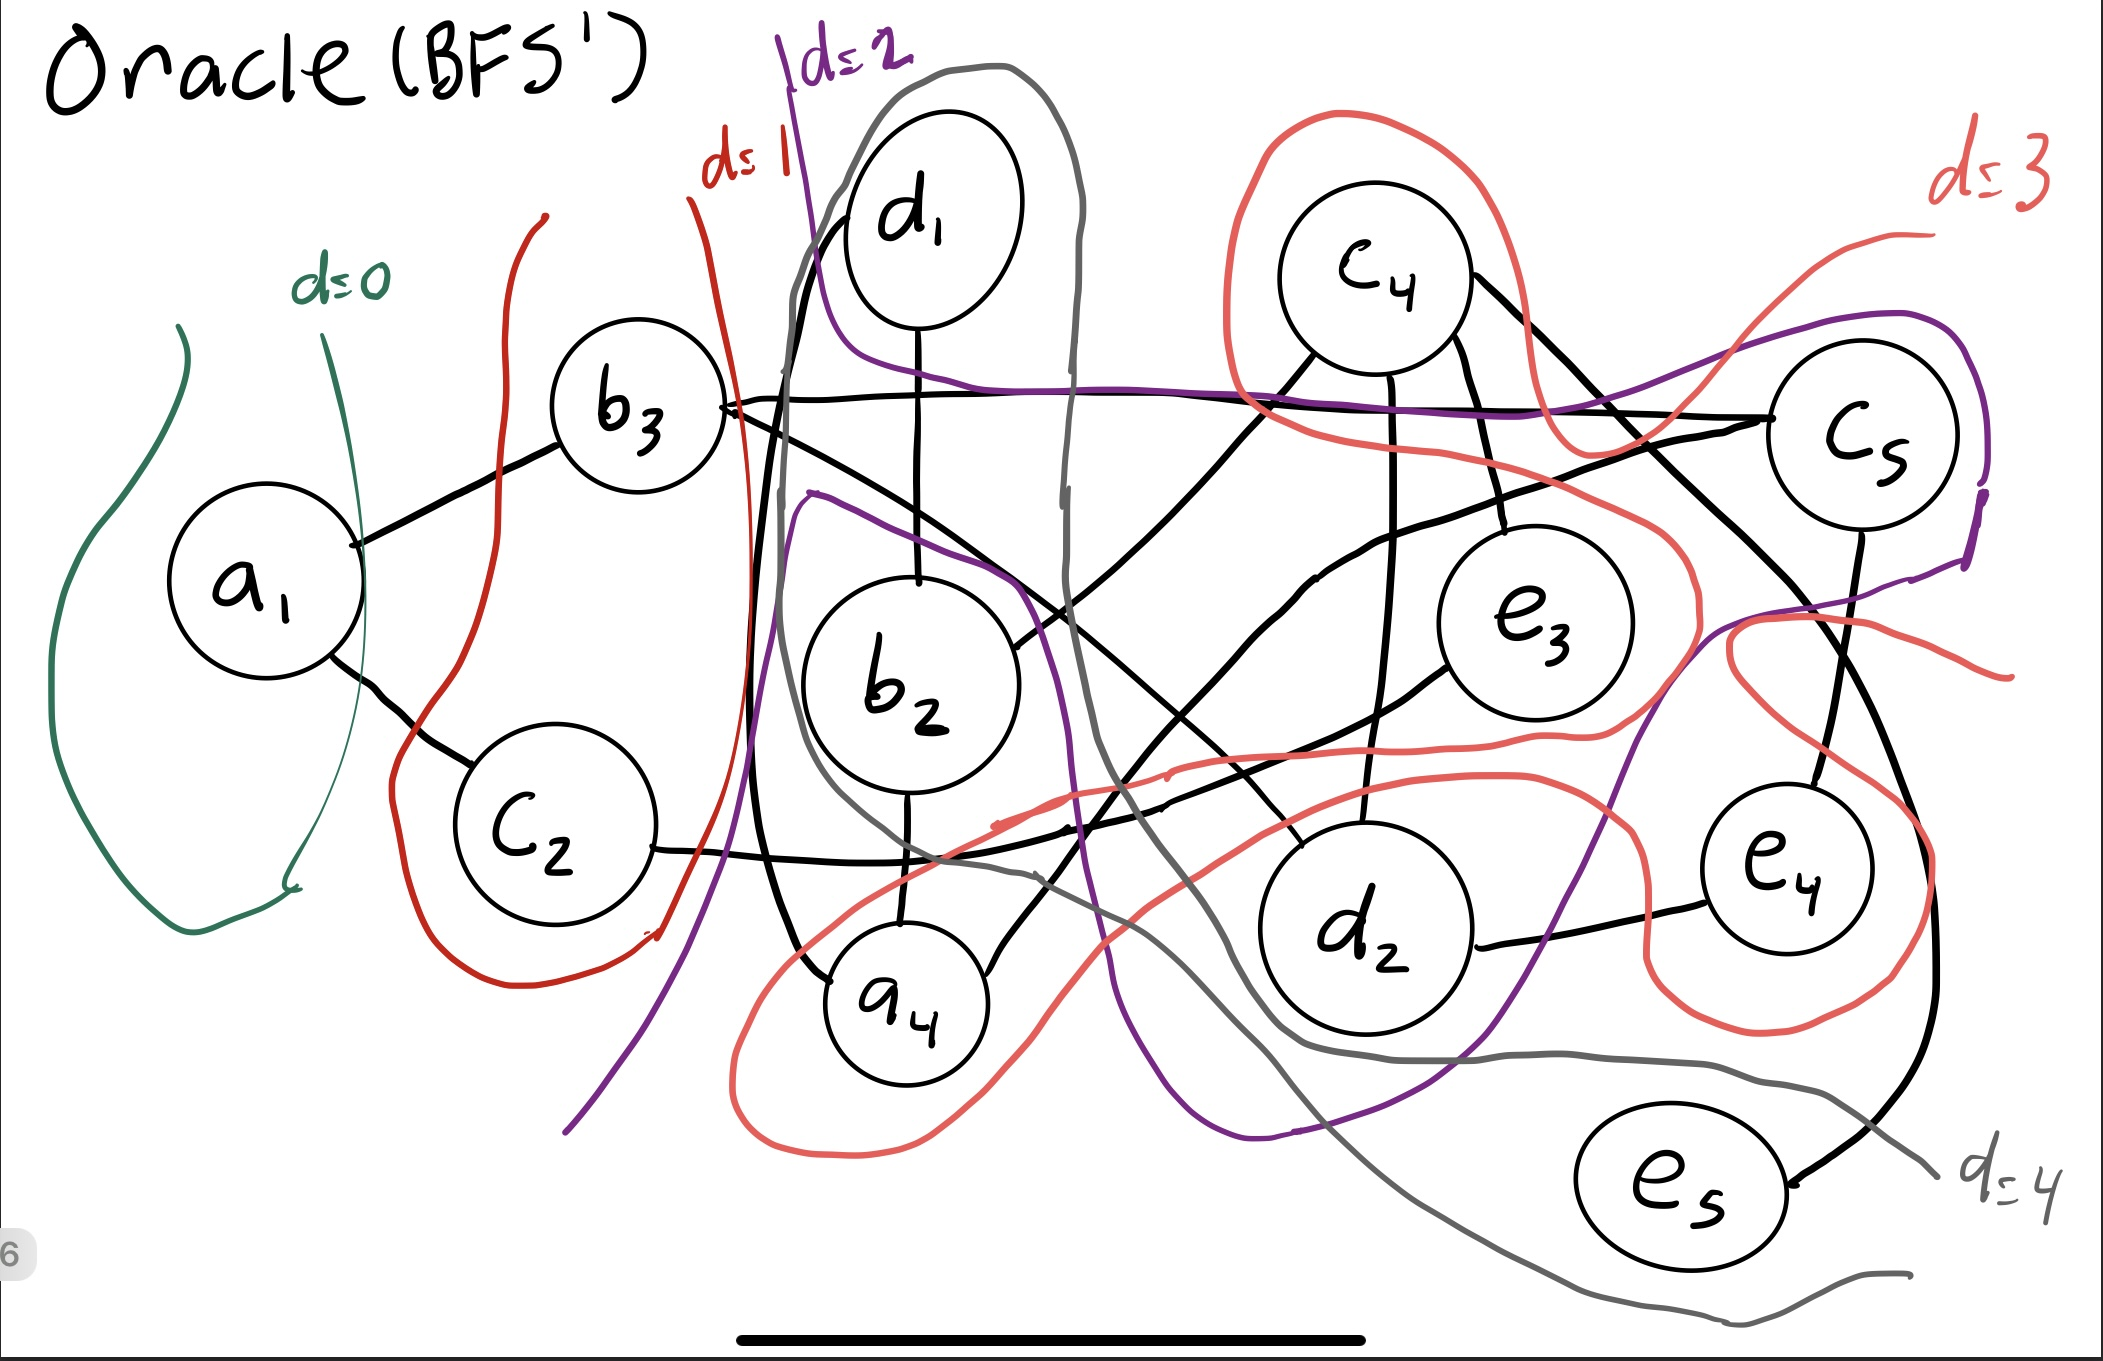
\includegraphics[width=.75\linewidth]{IMG_0132.jpg}
    \caption{Oracle (frontiers)}
    \label{fig:oracle-frontiers}
\end{figure}

\begin{figure}[H]
    \centering
    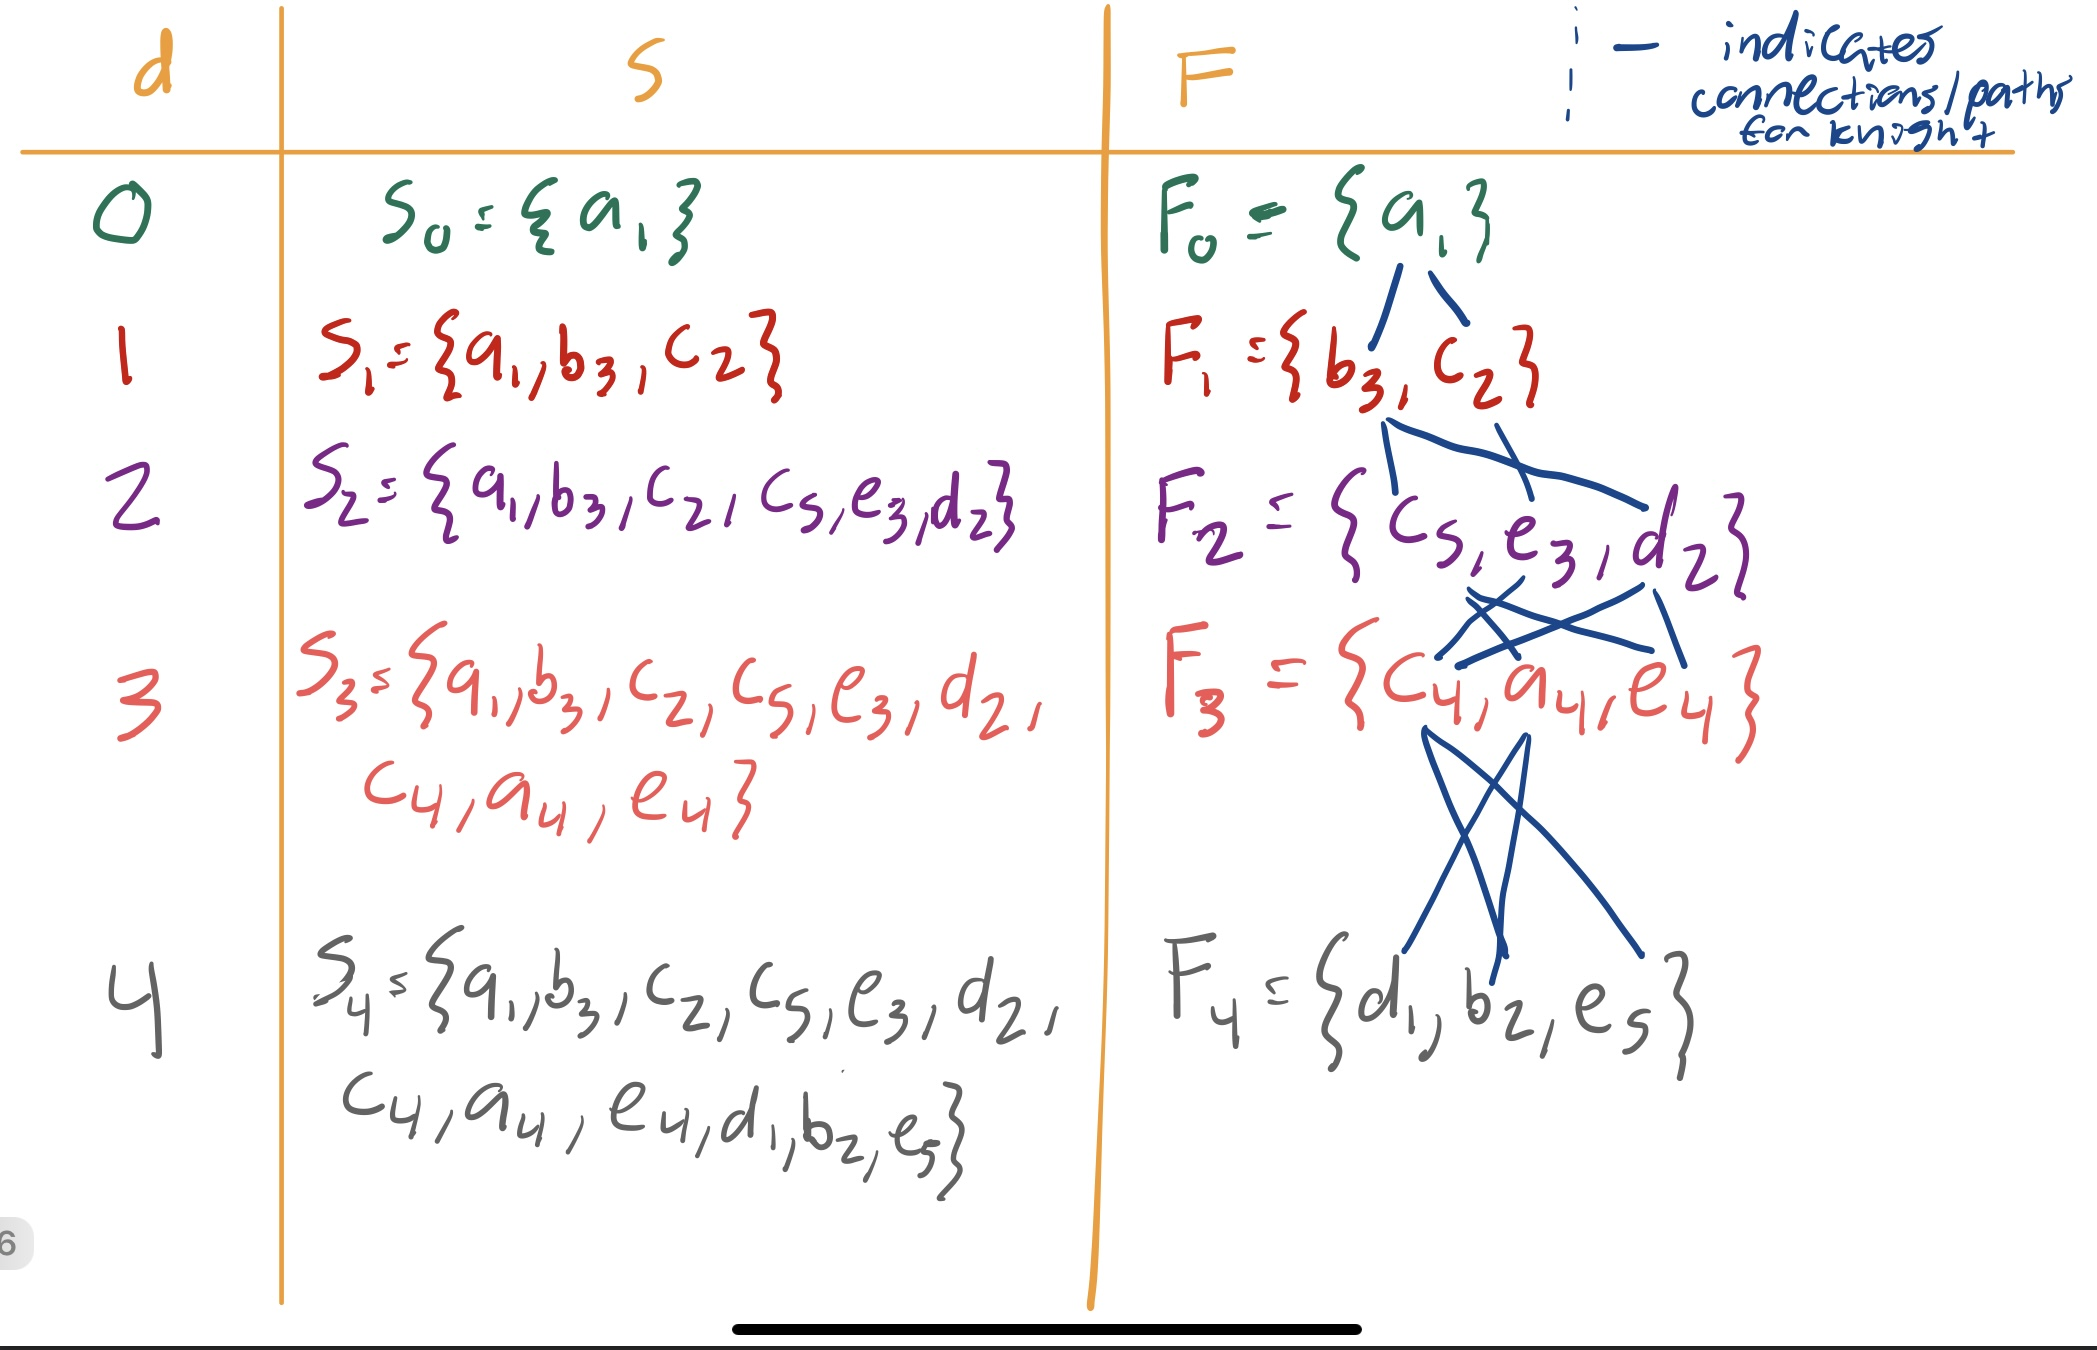
\includegraphics[width=.75\linewidth]{IMG_0133.jpg}
    \caption{Oracle (table)}
    \label{fig:oracle-table}
\end{figure}

\begin{figure}[H]
    \centering
    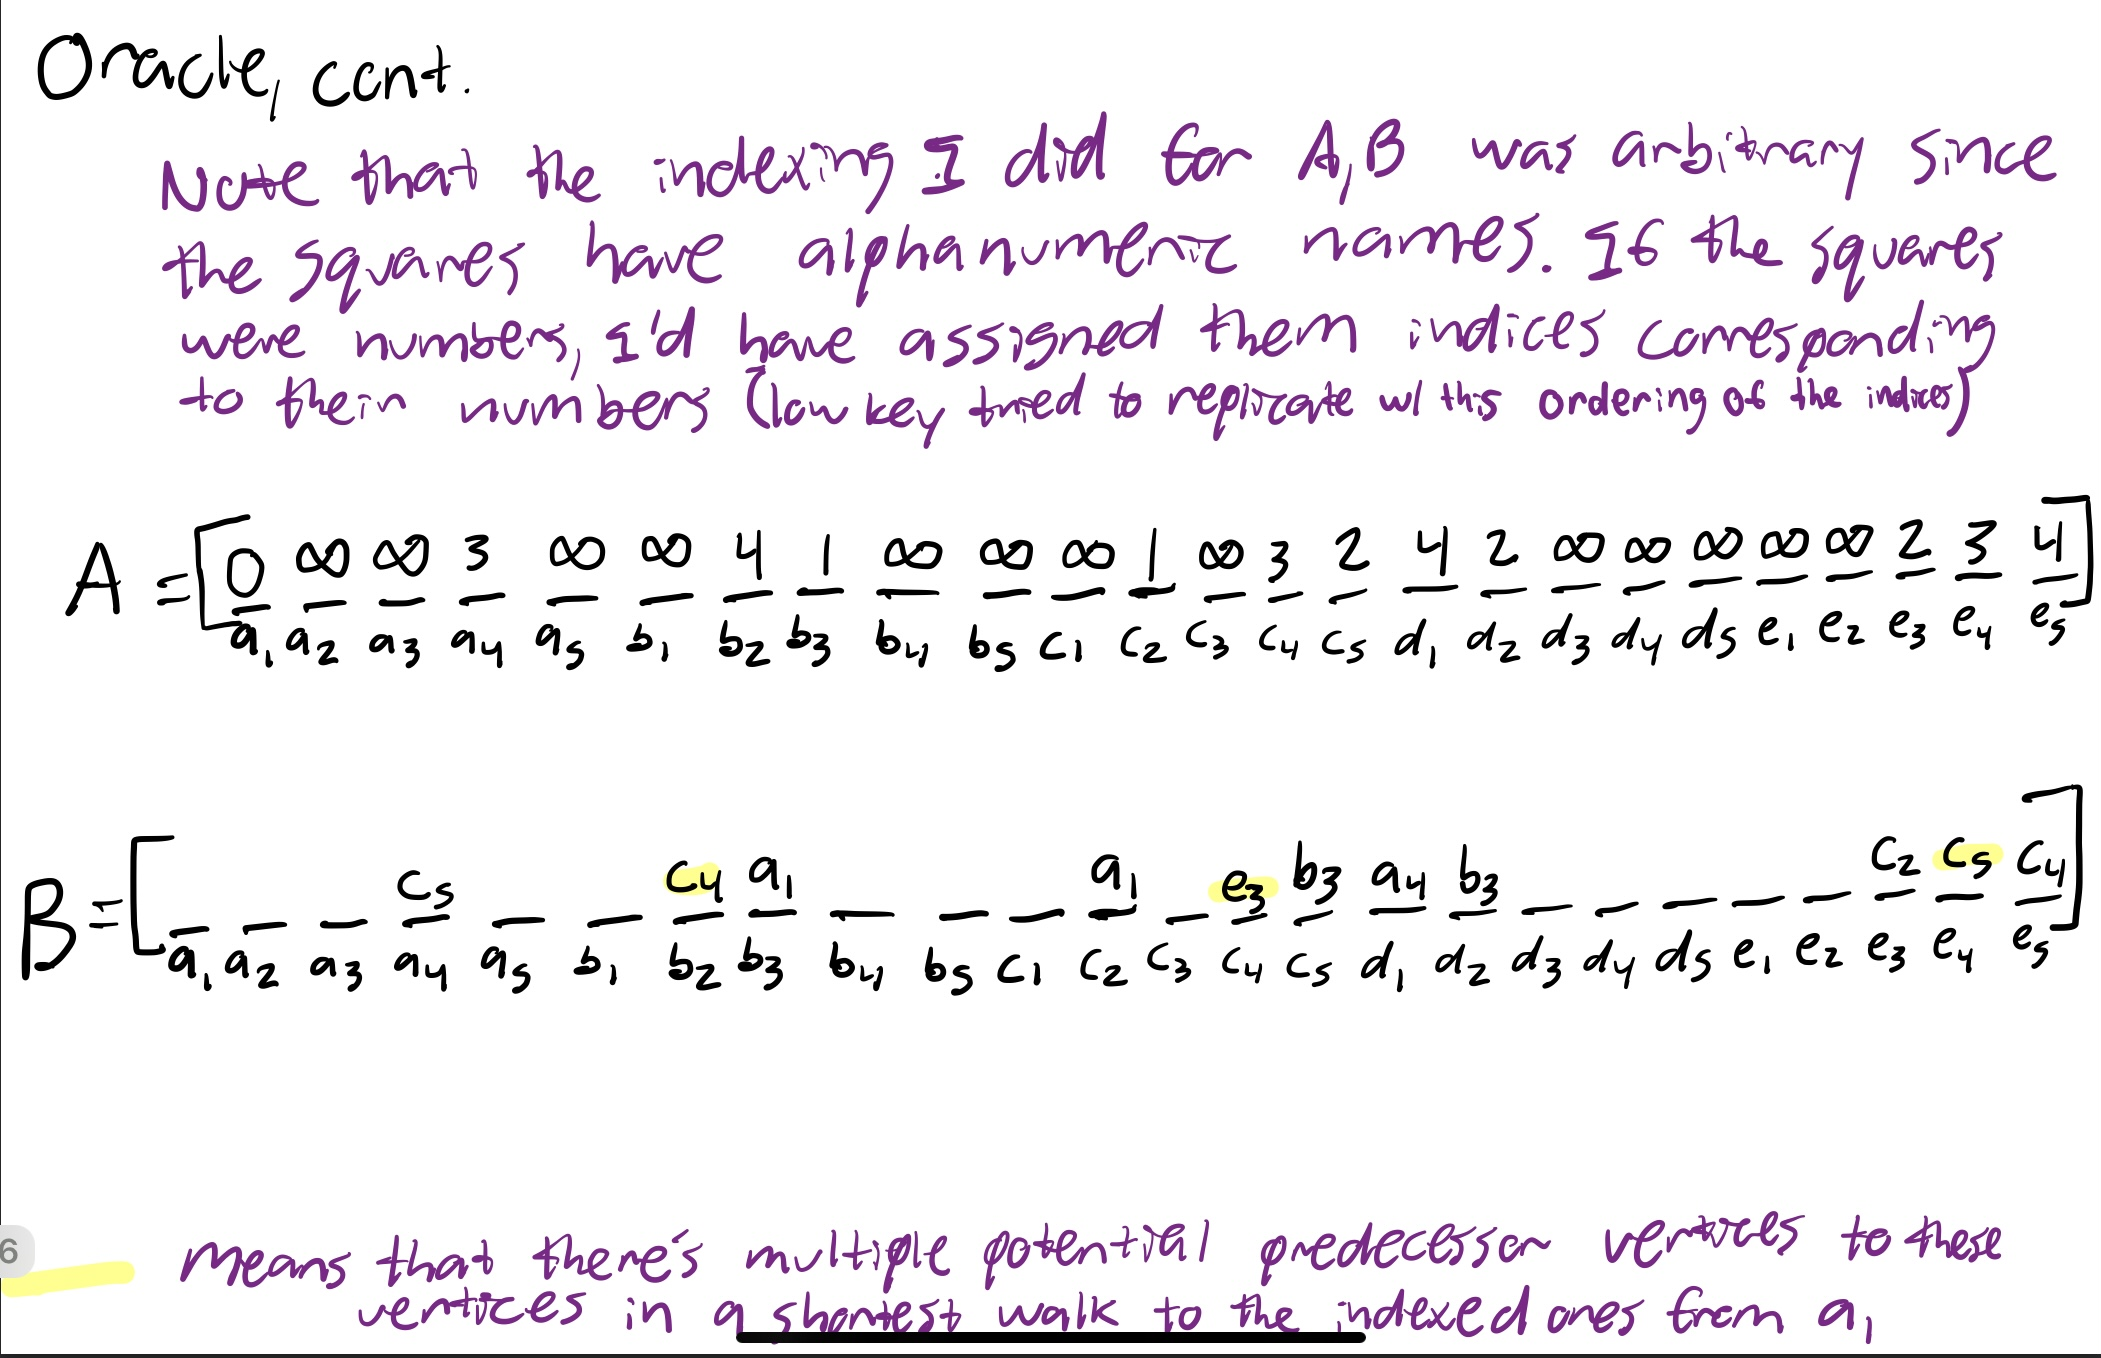
\includegraphics[width=.75\linewidth]{IMG_0134.jpg}
    \caption{Oracle (arrays)}
    \label{fig:oracle-arrays}
\end{figure}

\begin{figure}[H]
    \centering
    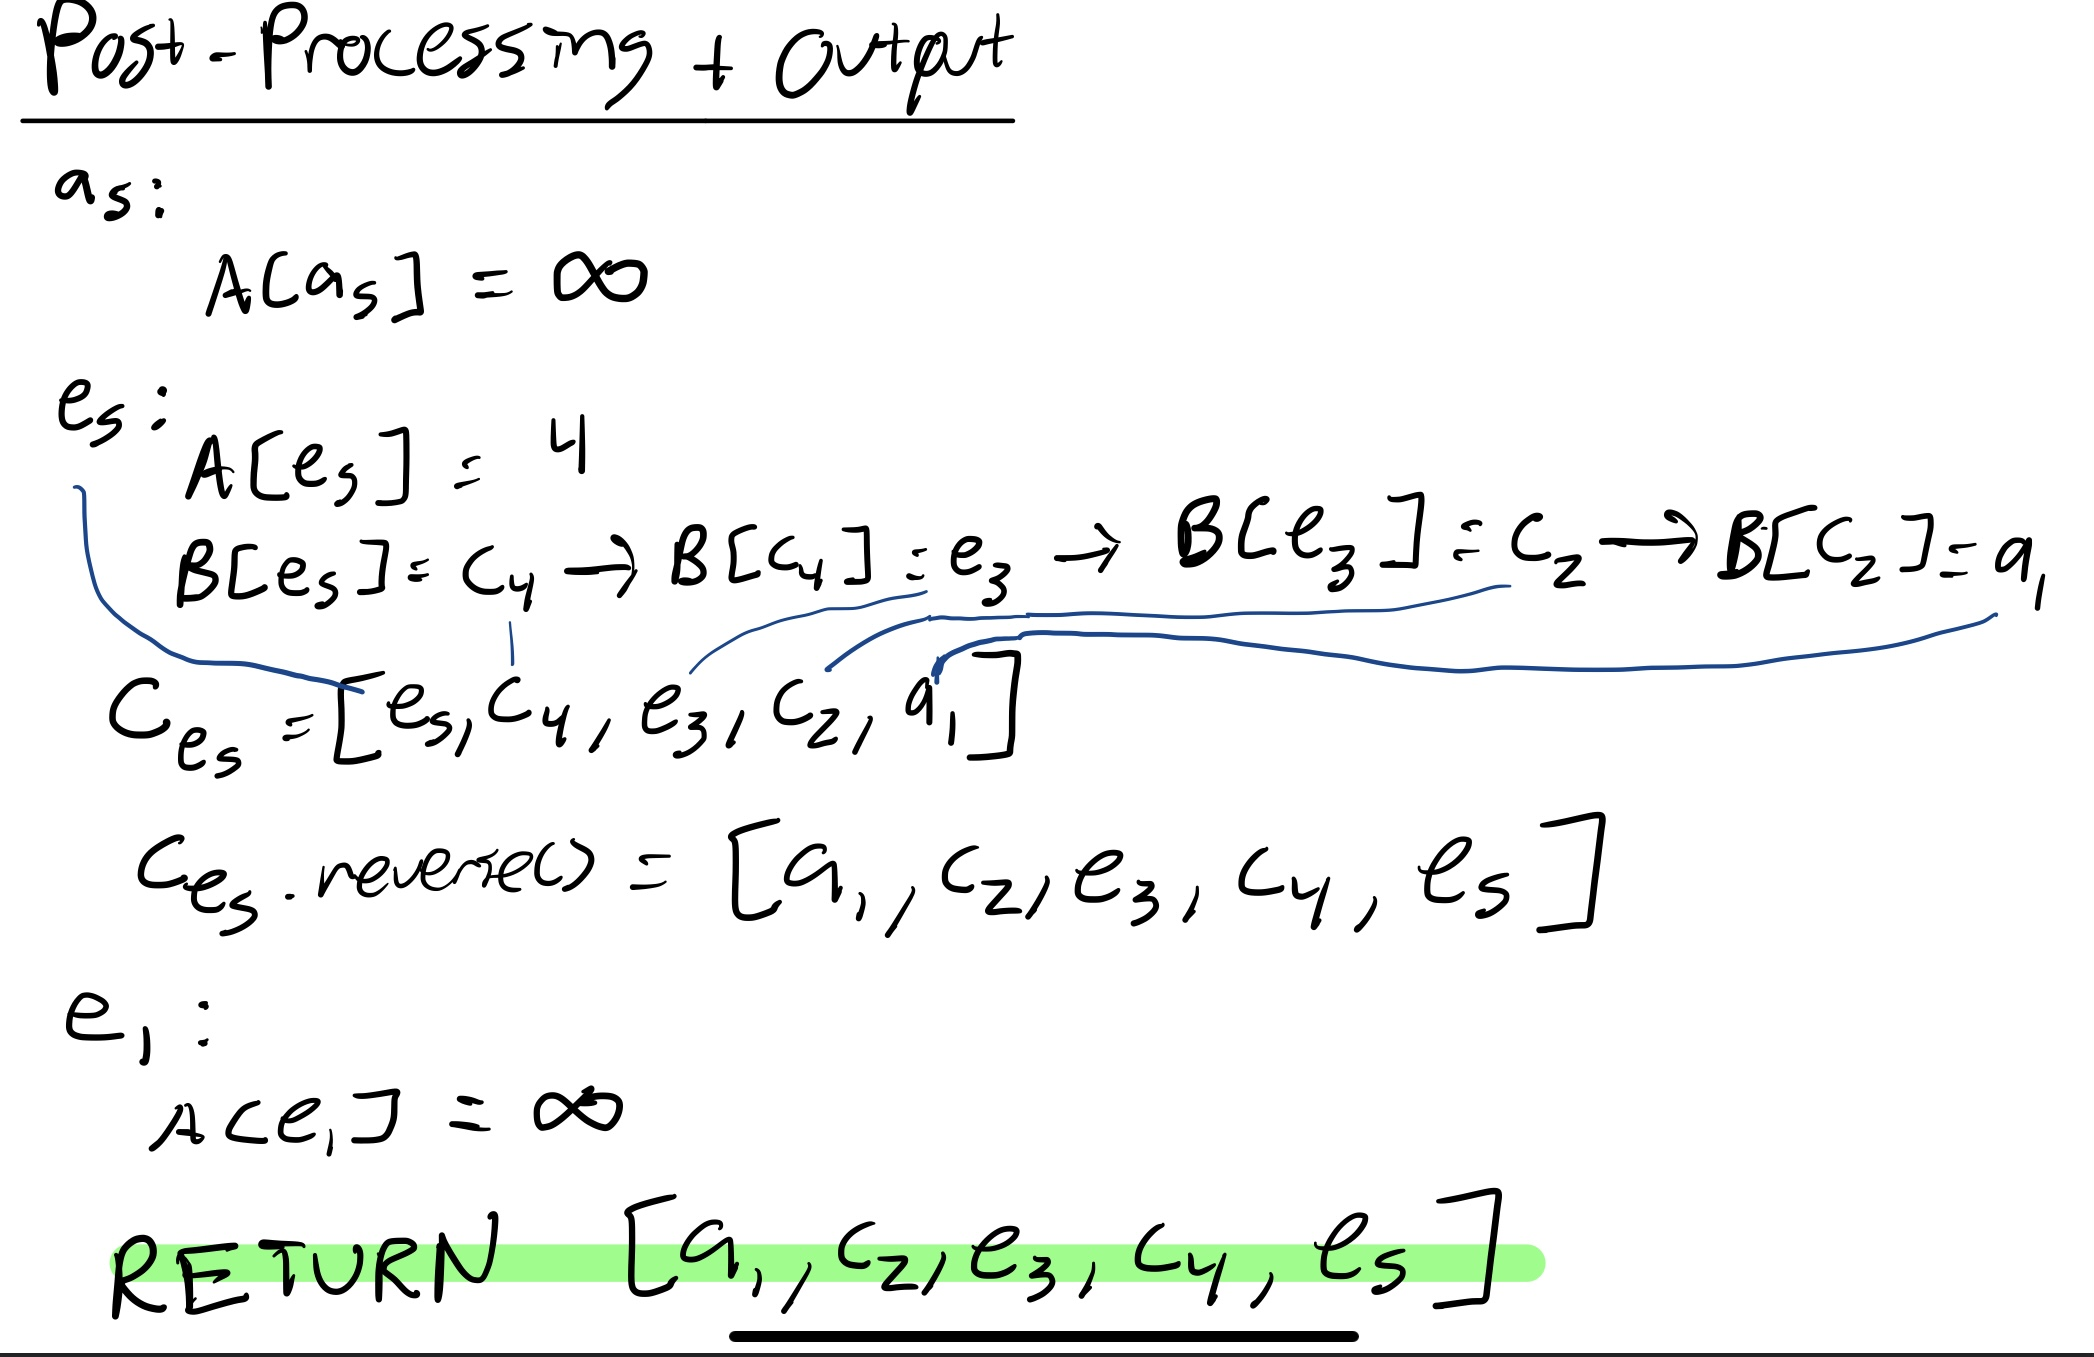
\includegraphics[width=.75\linewidth]{IMG_0135.jpg}
    \caption{Postprocess}
    \label{fig:postprocess}
\end{figure}


 \item (Maximal Independent Sets) \label{prob:maximalIS} Let $G=(V,E)$ be a graph.  A set $S\subseteq V$ is a {\em maximal} independent set if we cannot add any vertices to $S$ while it remains an independent set.  That is, for every vertex $v\in V\setminus S$, $S\cup\{v\}$ is not an independent set.
    \begin{enumerate}
        \item Show that given a graph $G$, a maximal independent set can be found in time $O(n+m)$.  Note that this is in sharp contrast to {\em maximum-size} independent sets, for which we do not know any subexponential-time algorithms. (Hint: be greedy.) \\

        \textbf{Rosh's Greedy Alg}

\begin{enumerate}
    \item Start with the set $V$ in $G$ containing all vertices of the graph, and an empty set called $S$.
    \item Choose an arbitrary vertex $v$ in $V$, and find an independent set $U$ containing $v$.
    \item For all the vertices $u$ in $U$:
    \begin{itemize}
        \item Add $u$ to the set $S$.
        \item Remove all vertices in $U$ from $V$ and their incident edges from $E$.
        \item Remove all vertices $z$ that are neighbors of any vertex in $U$ from $V$ and their incident edges from $E$.
    \end{itemize}
    \item Repeat steps ii-iii until $V = \emptyset$.
    \item return $S$, the maximal independent set
\end{enumerate} \\
\textbf{Correctness:} S is a maximal independent set because it contains a set of vertices in G that form an independent set, but wouldn't retain the independent set property if any additional vertices in G were to be added to S. We know this is the case because we only add vertices to S that aren't adjacent to the vertices already in S, as adjacent vertices to the ones in S are removed from V along with all their edges from E. Since we're carrying out the process until $V = \emptyset$, we ensure that all vertices not adjacent to those already in S will be put into S. Thus, S is a maximal independent set because no other vertices can be added to the set without breaking the independent set property. \\

\textbf{Runtime Justification:} Essentially, this algorithm looks over every vertex in V and every edge in E. We know this because the algorithm goes on till $V = \emptyset$, meaning all vertices and edges have been deleted from the graph G. For each look at a vertex/edge, a constant number of operations is performed (to remove the vertex/edge from the graph, add the vertex to S). Specifically, each vertex is processed once, and each edge is removed once one of its incident vertices are removed. Thus, the algorithm operates in a runtime on the order of the total number of vertices and edges in G, or $O(n+m)$. \\
        
        \item Show that if $G$ is 3-colorable, then it has a 3-coloring $f$ in which the set of vertices of color 2 (i.e. $f^{-1}(2)$) is a maximal independent set. \\

\textbf{Bruh this statement isn't even true in a graph containing $\geq$ 3 vertices with no edges. I assume you want me to show it for non-degenerate graphs, so I'll show the statement is true for graphs that are at minimum 2-colorable:} \\

If G is a valid, arbitrarily 3-colorable graph, the following algorithm will yield a valid 3-coloring of G where the set of vertices of color 2 forms a maximal independent set.

\begin{enumerate}
    \item Initialize: Let each vertex in $G$ have no color initially, or start with the existing 3-coloring if one exists. 
    \item For each vertex $v$ in $V$ of $G$:
    \begin{itemize}
    \item Ensure the vertex is of color 2 whenever possible. We can use a simple greedy coloring approach to do this:
        \begin{itemize}
            \item If $v$ is already assigned color 2, skip to the next vertex.
            \item Check if any of $v$'s neighbors are assigned color 2.
            \item If none of $v$'s neighbors are assigned color 2, assign color 2 to $v$.
    \end{itemize}
    \end{itemize}
    
    
    \item For each vertex $v'$ not assigned color 2:
    \begin{itemize}
        \item Assign the vertex color 1 or color 3 such that no two adjacent vertices share the same color. We can use a simple greedy coloring approach to do this:
            \begin{itemize}
                \item Look at the colors of all of neighbors of $v'$.
                \item Assign $v'$ a color \textbf{not} used by its neighbors from {color 1, color 3}.
            \end{itemize}
     \item If a situation arises where the vertices that aren't colored color 2 are all colored either color 1 or color 3 (AKA, a two colored graph because G happens to be both 3 and 2-colorable), make sure to reassign the unused third color to at least one of those vertices so the graph is 3-colored. This is unlikely to happen, but it could with a graph where $\forall v'$, $v'$ has neighbors only of color 2.
    \end{itemize} 
    \item Return the 3-coloring of $G$, where the set of vertices assigned color 2 forms a maximal independent set.
\end{enumerate} \\

\textbf{Proof of Correctness:} After running this algorithm that potentially recolors G, we end up with a graph in which all vertices that aren't of color 2 are connected to a vertex of color 2. This occurs due to us assigning color 2 to every eligible vertex. Thus, the vertices colored color 2 form a maximal independent set because none of the other-colored vertices can be colored 2 without us having adjacent color-2 vertices (a violation of the independent set property). The algorithm also makes sure our coloring is a 3-coloring, handling interesting cases where our G was both 2-colorable and 3-colorable by making sure to assign the missing third color to at least one of the vertices not colored color 2. \\

        \item It is known that every graph $G$ has at most $3^{n/3}$ maximal independent sets, and there is an algorithm (the Bron-Kerbosch algorithm) that enumerates all of the maximal independent sets in time $O(3^{n/3}).$  Use this fact to conclude that 3-coloring can be solved in time $O((n+m)\cdot 3^{n/3}) = O(1.44^n),$ improving the runtime of $O(1.89^n)$ from SRE4. \\

        Per what's given, we know there's at most $3^{\frac{n}{3}$ maximal independent sets in a graph G with $n$ vertices. Using this, we can achieve 3-coloring as follows: \\
        
\begin{enumerate}
    \item Use Bron-Kerbosch to enumerate all of the maximal independent sets.
    \item For each maximal independent set $S$ in the list of maximal independent sets:
    \begin{itemize}
        \item Color all vertices in $S$ with one color.
        \item Temporarily remove all vertices and edges incident to vertices in $S$ from the graph (but store them for later use).
        \item Run BFSColoring($G'$), where $G'$ is $G$ without vertices or edges incident to vertices in $S$ and the two colors are different from the one assigned to vertices in $S$.
        \item If BFSColoring($G'$) detects some error (i.e., $G'$ isn't 2-colorable):
        \begin{itemize}
            \item Break from the loop and try again with the next maximal independent set in the list.
        \end{itemize}
        \item Else:
        \begin{itemize}
            \item It means $G'$ is 2-colorable.
            \item Re-insert the vertices and edges incident to the vertices in $S$ back into $G'$ so we essentially have $G$ again.
            \item Return the now 3-colored graph.
        \end{itemize}
    \end{itemize}
\end{enumerate} \\

        \textbf{Correctness:} Similar to 2b), as there exists a 3-coloring in a 3-colorable graph where the maximal independent set vertices for some maximal independent set in our list can all get one color and the remaining part of the graph can be colored in 2 colors. \\

       \textbf{Runtime:}
        Using Bron-Kerbosch takes $O(3^{\frac{n}{3}})$ time. We have to iterate over at worst $3^{\frac{n}{3}}$ maximal independent sets. Searching for a 3-coloring of G in each iteration takes $O(x) + O(x) + O(b) + O(n-x + m-b) + O(x) + O(b) = O(n+2x+m+b)$, where $x$ is the number of vertices in S and $b$ is the number of edges incident to those vertices. It must be the case that $x = O(n)$ and $b = O(m)$ due to the fact the independent set can't contain more vertices or have more incident edges than the graph. Thus, each iteration through a maximal independent set in the list takes $O(n+2n + m + m) = O(3n + 2m) = O(n + m)$ time.
        Aggregating, we see that the total 3-coloring runtime takes $O(3^{\frac{n}{3}}) + O(3^{\frac{n}{3}})\cdot O(n + m) = O(3^{\frac{n}{3}}) \cdot O(n + m + 1) = O(3^{\frac{n}{3}}) \cdot O(n + m) = O(3^{\frac{n}{3}} \cdot (n + m))$ time. Boom shackalaka.
        
        
    \end{enumerate}
 
 \item (Exponential-Time Coloring) 
  In the \href{https://github.com/Harvard-CS-120/cs120/tree/main/fall2022/psets}{Github repository} for PS5, we have given you basic data structures for graphs (in adjacency list representation) and colorings, an implementation of the Exhaustive-Search $k$-Coloring algorithm, 
  an implementation of the Bron-Kerbosch algorithm, and a variety of test cases (graphs) for coloring algorithms. 

  \begin{enumerate}
      \item Implement the $O(n+m)$-time algorithm for 2-coloring that we covered in class in the function \texttt{bfs\_2\_coloring}, verifying its correctness by running \texttt{python3 -m ps5\_tests 2}.
        Your implementation of BFS should follow the presentation and notation that we used in class (with the loop over distance $d$ and the sets $F$ and $S$), which may be different than presentation of BFS in other sources (online or in the optional textbooks). \\

        In code \\

      \item Implement the $O((n+m)\cdot 3^{n/3})$-time algorithm for 3-coloring (MaximalIS + BFS) from Problem~\ref{prob:maximalIS} above in the function \texttt{iset\_bfs\_3\_coloring}, also verifying its correctness by running \texttt{python3 -m ps5\_tests 3}. \label{part:TbT} \\

      In code \\
    
    \item Compare the efficiency of Exhaustive-Search 3-coloring and the $O((n+m)\cdot 3^{n/3})$-time algorithm. Specifically, identify and write down the largest instance size $n$ each algorithm is able to solve (within a time limit you specify, e.g. 1 second) and the smallest instance size $n$ each algorithm is unable to solve (again within that same time limit). 
    
    In addition to these numeric values, please provide a brief explanation of why these results make sense, based on your knowledge of both the algorithms' runtime and how each algorithm goes about finding a coloring. For this part, there is no need to go through every combination of parameters; feel free to give just the largest and smallest instances each algorithm can solve and speak generally as to why one algorithm performs better than the other. More instructions can be found in \texttt{ps5\_experiments}. \\

    Size Matters:) I was low key gassed so I didn't adjust the adjustable parameters this is just based off of what the default experiment file returned. \\

    \textbf{Exhaustive-Search 3-coloring:} \\
    
    largest observed instance size $n$ solvable within 1 second: $\approx$ 20 (in the randomized cluster collections) \\
    smallest observed instance $n$ unsolvable within 1 second: $\approx$ 36 (in the randomized cluster collections) \\

    \textbf{ISET-BFS 3-coloring:} \\

    largest observed instance size $n$ solvable within 1 second: $\approx$ 1000 (in the rings) \\
    smallest observed instance $n$ unsolvable within 1 second: $\approx$ 40 (in the randomized cluster with low edge probability) \\

    Generally, ISET-BFS 3-coloring which has runtime ($O((n+m)\cdot 3^{n/3})$) outperforms Exhaustive-Search 3-coloring which has runtime $O(3^n)$. This makes sense because ISET-BFS 3-coloring methodically colors the graph spreading along edges whereas Exhaustive-Search 3-coloring naively goes through all the possible permutations of colorings (valid or invalid) of a graph. \\

    In the ring examples, Exhaustive-Search 3-coloring flopped but ISET-BFS 3-coloring was able to solve all of them. It makes sense because Exhaustive-Search 3-coloring has to brute force through an explosive number of random combinations that are unlikely to be valid 3-colorings due to the rings' structures, whereas ISET-BFS 3-coloring methodically uses maximal independent sets to make the coloring process much more efficient (and rings also generally just have fewer unique maximal independent sets). \\

    In the clusters examples with varying edge probability, we I noticed that ISET-BFS 3-coloring was more adversely impacted by lower edge probabilities that Exhaustive-Search 3-coloring (makes sense because then there's a higher chance the graphs aren't as connected, leading to more existing maximal independent sets that need to be looped over). Still, that "probability of edge effect" was relatively trivial because ISET-BFS 3-coloring always outperformed Exhaustive-Search 3-coloring, especially as $n$ grew. Size increases hurt each algorithm's runtime regardless (ISET-BFS 3-coloring didn't run on time with $n = 72$ even with higher edge probabilities).
    
  \end{enumerate}
  
  

\item (Reflection): Take one homework problem you have worked on this semester that you struggled to understand and solve, and explain how the struggle itself was valuable.  In the context of this question, describe the struggle and how you overcame the struggle. You might also discuss whether struggling built aspects of character in you (e.g. endurance, self-confidence, competence to solve new problems) and how these virtues might benefit you in later ventures. 

 \textit{Note: As with the previous psets, you may include your answer in your PDF submission, but the answer should ultimately go into a separate Gradescope submission form.}

 \textit{Quick note on grading: Good responses are usually about a paragraph, with something like 7 or 8 sentences. Most importantly, please make sure your answer is specific to this class and your experiences in it. If your answer could have been edited lightly to apply to another class at Harvard, points will be taken off.}

\item Once you're done with this problem set, please fill out \href{https://forms.gle/pR1Mt4PmMhUfuW1G6}{this survey} so that we can gather students' thoughts on the problem set, and the class in general. It's not required, but we really appreciate all responses!
\end{enumerate}

\end{document}